\chapter{مطيافية الكتلة والمطيافية الذرية}\label{ch:b2:mass-spec-atomic}

الألعاب النارية حمراء بأملاح السترونشيوم، وخضراء بأملاح الباريوم، وصفراء بالصوديوم: فاللهب يحوّل
الذرات إلى ضوء بألوان تدل على هويتها. ومطياف الكتلة، الأكثر تواضعًا في مظهره،
يزن الجزيئات فرادى، ويفرزها بحسب نظائرها ويكسرها إلى قطع تخبر كتلها
كيف بُنيت. وكلتا التقنيتين تجيب عن السؤال «ما الذي في هذه العينة، وكم مقداره؟»
انطلاقًا من كميات صغيرة جدًا، الأولى للجزيئات، والثانية للعناصر.

\begin{omfigure}

\includegraphics[width=0.58\linewidth]{images/book3/ai/b2-32-fireworks.jpg}

{\small ألعاب نارية فوق نهر (رسم توضيحي). أصفر الصوديوم هو ضوء ذراته؛ أما
الأحمر والأخضر الداكنان فمصدرهما في الغالب جزيئات صغيرة للسترونشيوم والباريوم تتكوّن في اللهب.}
\end{omfigure}

\begin{recall}
المجلد المدرسي: النظائر ووفرتها. ومجلد السنة الأولى: مستويات الطاقة والخطوط
الطيفية، والامتصاصية وقانون بير--لامبرت، والكاتيونات الكربونية والجذور، ودرجة عدم التشبع.
و\cref{ch:b2:chromatography}: \omterm{def:b2:chromatography:techniques}{كروماتوغرافيا الغاز}، التي كثيرًا ما تغذي مطياف كتلة.
\end{recall}

\section{مطياف الكتلة}

\begin{definition}[مطيافية الكتلة]\label{def:b2:mass-spec-atomic:spectrum}
\emph{مطيافية الكتلة}\index{مطيافية الكتلة} تحوّل جزيئات العينة إلى أيونات غازية،
وتفصل الأيونات بحسب \emph{نسبة الكتلة إلى الشحنة}\index{نسبة الكتلة إلى الشحنة} $m/z$
(الكتلة بوحدات الكتل الذرية الموحدة مقسومة على عدد الشحنات) وتعدّها. 
و\emph{طيف الكتلة}\index{طيف الكتلة} يرسم وفرة الأيونات بدلالة $m/z$، عادة على هيئة
شدات نسبية؛ وقمته الأشد، المثبتة عند 100، هي \emph{قمة الأساس}\index{قمة الأساس}.
\end{definition}

للمطياف ثلاثة أجزاء. يصنع المصدر الأيونات. ففي التأين الإلكتروني (EI) يعبر بخار
العينة حزمة من الإلكترونات طاقتها \qty{70}{eV}، تنتزع إلكترونًا من الجزيئات 
وتتركها بطاقة زائدة، فيتفكك كثير منها. وفي التأين بالرذاذ الكهربائي (ESI) يُرش محلول
من إبرة مشحونة؛ وحين تتبخر القطيرات، تغادرها الجزيئات حاملة بروتونًا إضافيًا
(أو أيون صوديوم)، سليمة: وهي الطريقة المفضلة للجزيئات الكبيرة الهشة. ثم يفرز المحلل
الأيونات، ويعدّها كاشف.

\begin{omfigure}
\begin{tikzpicture}[x=1cm, y=1cm]
\draw[black!70, fill=omDef!10, rounded corners=2pt] (0,-0.6) rectangle (1.6,0.6);
\node[font=\small, align=center] at (0.8,0) {مصدر\\الأيونات};
\draw[black!70] (2.0,-0.7) -- (2.0,0.7); \draw[black!70] (2.4,-0.7) -- (2.4,0.7);
\node[font=\footnotesize] at (2.2,1.0) {\foreignlanguage{arabic}{شبكات، $U$}};
\draw[black!70] (2.6,-0.5) rectangle (8.4,0.5);
\node[font=\small] at (5.6,0.8) {\foreignlanguage{arabic}{أنبوب انجراف خالٍ من المجال، طوله $L$}};
\draw[black!70, fill=black!15] (8.5,-0.6) rectangle (8.8,0.6);
\node[font=\small, align=center] at (9.6,0) {كاشف};
\foreach \x/\c in {3.4/omThm, 4.6/omDef, 6.3/omMeth}{\fill[\c] (\x,0) circle (0.1);}
\draw[->, thick] (6.6,0) -- (7.4,0);
\node[font=\footnotesize, align=center] at (5.5,-0.85) {\foreignlanguage{arabic}{الأيونات الخفيفة تسبق، والثقيلة تتأخر}};
\end{tikzpicture}
\par\vspace{4pt}

{\small محلل زمن الطيران (رسم تخطيطي). الأيونات المسرَّعة عبر فرق الجهد نفسه
$U$ تخرج بالطاقة الحركية نفسها؛ وفي أنبوب الانجراف تسير الأخف أسرع وتبلغ
الكاشف أولًا.}
\end{omfigure}

\begin{proposition}[زمن الطيران]\label{prop:b2:mass-spec-atomic:time-of-flight}
الأيون ذو الكتلة $m$ والشحنة $ze$، المسرَّع من السكون عبر فرق جهد $U$، يعبر
أنبوبًا خاليًا من المجال طوله $L$ في
\begin{equation*}
t = L\sqrt{\frac{m}{2zeU}}:
\end{equation*}
فيزداد زمن الطيران كالجذر التربيعي للنسبة $m/z$.
\end{proposition}

\begin{proof}
انحفاظ الطاقة في مجال التسريع يعطي $\tfrac12mv^2 = zeU$، إذن $v = \sqrt{2zeU/m}$، 
ويُعبر الأنبوب بسرعة ثابتة: $t = L/v$.
\end{proof}

وتفرز محللات أخرى الأيونات بطرق مختلفة: فرباعي الأقطاب لا يمرر إلا أيونات قيمة واحدة للنسبة $m/z$ في كل مرة،
تُختار بجهود متذبذبة على أربعة قضبان؛ والقطاع المغناطيسي يحني الأيونات على دوائر يتعلق نصف قطرها
بزخمها. وفيها كلها لا يُقاس إلا $m/z$؛ ومعظم الأيونات التي يصنعها EI تحمل شحنة
واحدة، فتكون $m/z$ هي كتلتها ببساطة.

\section{الأيون الجزيئي}

\begin{definition}[الأيون الجزيئي وأيونات الشظايا]\label{def:b2:mass-spec-atomic:molecular-ion}
\emph{الأيون الجزيئي}\index{أيون جزيئي} $\mathrm M^{+\bullet}$ هو الكاتيون الجذري المتكوّن حين
يفقد جزيء إلكترونًا واحدًا؛ و$m/z$ له هي الكتلة المولية للجزيء المكوّن من النظائر الأوفر
وجودًا. و\emph{أيون الشظية}\index{أيون شظية} ينشأ من الأيون الجزيئي بانكسار
روابط.
\end{definition}

يعطي \omterm{def:b2:mass-spec-atomic:molecular-ion}{الأيون الجزيئي} الكتلة الجزيئية، أول حقيقة عن المجهول. وهو أحيانًا ضعيف أو
غائب في EI، حين يتكسر \omterm{def:b2:mass-spec-atomic:molecular-ion}{الأيون الجزيئي} بسهولة مفرطة؛ وعندئذ يؤكده الرذاذ الكهربائي، الذي يعطي $[\mathrm M +
\mathrm H]^+$ أعلى بوحدة واحدة.

\begin{definition}[قاعدة النيتروجين]\label{def:b2:mass-spec-atomic:nitrogen-rule}
تنص \emph{قاعدة النيتروجين}\index{قاعدة النيتروجين} على أن للجزيء كتلة اسمية فردية (مجموع
الأعداد الكتلية لنظائره الأوفر وجودًا) إذا وفقط إذا حوى عددًا فرديًا من ذرات
النيتروجين.
\end{definition}

\begin{proposition}[صحة قاعدة النيتروجين]\label{prop:b2:mass-spec-atomic:nitrogen-rule}
تصح \omterm{def:b2:mass-spec-atomic:nitrogen-rule}{قاعدة النيتروجين} لكل جزيء بلا إلكترونات منفردة مبني من C وH وN وO وS 
والهالوجينات.
\end{proposition}

\begin{proof}
الكتل الاسمية زوجية للعناصر C (12) وN (14) وO (16) وS (32)، وفردية للعنصر H (1) وللهالوجينات (19،
35، 79، 127). والتكافؤات زوجية للعناصر C وO وS، وفردية للعناصر H وN والهالوجينات. وفي جزيء
بلا إلكترونات منفردة، تستعمل كل رابطة تكافؤًا واحدًا من كل من ذرتيها، فيكون مجموع كل
التكافؤات زوجيًا، ويكون عدد الذرات الفردية التكافؤ، $n_{\ce{H}} + n_{\ce{X}} + n_{\ce{N}}$،
زوجيًا. وزوجية الكتلة الاسمية هي زوجية $n_{\ce{H}} + n_{\ce{X}}$، فهي إذن زوجية
$n_{\ce{N}}$.
\end{proof}

\begin{definition}[النمط النظائري]\label{def:b2:mass-spec-atomic:isotope-pattern}
\emph{النمط النظائري}\index{نمط نظائري} لأيون هو مجموعة القمم عند $M$، $M+1$،
$M+2$، \dots\ التي تنتجها الجزيئات الحاوية لنظائر أثقل، بشدات متناسبة مع
وفرة تلك الصور النظائرية.
\end{definition}

\begin{proposition}[القمة $M+1$]\label{prop:b2:mass-spec-atomic:m-plus-one}
من أجل أيون فيه $n_C$ ذرة كربون ولا عنصر آخر له نظير $+1$ معتبر،
\begin{equation*}
\frac{I(M+1)}{I(M)} \approx n_C\,\frac{a_{13}}{a_{12}} \approx n_C \times 1.1~\%,
\end{equation*}
حيث $a_{12} = 0.989$ و$a_{13} = 0.011$ الكسران الكميان لنظيري الكربون.
% ledger: iso:C12, iso:C13
\end{proposition}

\begin{proof}
احتمال أن تكون كل ذرات الكربون، وعددها $n_C$، \ce{^{12}C} هو $a_{12}^{n_C}$؛ واحتمال أن تكون واحدة بالضبط
\ce{^{13}C} هو $n_C\,a_{13}a_{12}^{n_C - 1}$ (القانون الثنائي الحد). والنسبة $n_C\,a_{13}/a_{12}$، 
والمساهمات الأخرى (ذرتا \ce{^{13}C}، \ce{^2H}، \ce{^{15}N}) أصغر بعامل من رتبة
$a_{13}$ أو أقل.
\end{proof}

\begin{proposition}[الكلور والبروم]\label{prop:b2:mass-spec-atomic:halogen-patterns}
من أجل أيون فيه $p$ ذرة كلور و$q$ ذرة بروم، تكون شدات $M$، $M+2$، $M+4$، \dots\
معاملات نشر $(a_{35} + a_{37}x)^p(a_{79} + a_{81}x)^q$ بقوى $x$، حيث تمثل كل
قوة للمتغير $x$ وحدتي كتلة. ومع $a_{35} = 0.758$، $a_{37} = 0.242$، $a_{79} = 0.5069$ 
و$a_{81} = 0.4931$، تعطي ذرة كلور واحدة $M : M+2 \approx 3 : 1$ وذرة بروم واحدة $\approx 1 : 1$.
% ledger: iso:Cl35, iso:Cl37, iso:Br79, iso:Br81
\end{proposition}

\begin{proof}
كل ذرة هالوجين هي، باستقلال، النظير الخفيف أو الثقيل، الذي يضيف 2 إلى الكتلة. 
واحتمال عدد معين $j$ من الذرات الثقيلة هو معامل $x^j$ في جداء عامل واحد
لكل ذرة، وهو النشر المذكور (القانون الثنائي الحد، لكل عنصر).
\end{proof}

\begin{omfigure}
\pgfplotsset{clu/.style={width=0.25\linewidth, height=3.3cm, ybar, bar width=5pt, ymin=0, ymax=118,
  xmin=-1.2, xmax=5.2, xtick={0,2,4}, xticklabels={$M$,$M\!+\!2$,$M\!+\!4$},
  tick label style={font=\tiny}, ytick=\empty, axis x line=bottom, axis y line=none,
  title style={font=\small, yshift=-4pt}, nodes near coords, nodes near coords style={font=\tiny},
  point meta=y, every node near coord/.append style={/pgf/number format/fixed, /pgf/number format/precision=0}}}
\begin{tikzpicture}
\begin{axis}[clu, title={\babelsublr{Cl}}]
\addplot[fill=omDef!55, draw=omDef, y filter/.expression={y==0 ? nan : y}] table[x=off, y=Cl] {figdata/out/bachelor-2-mass-spectra-a.dat};
\end{axis}
\end{tikzpicture}\hfill
\begin{tikzpicture}
\begin{axis}[clu, title={\babelsublr{Cl$_2$}}]
\addplot[fill=omDef!55, draw=omDef] table[x=off, y=Cl2] {figdata/out/bachelor-2-mass-spectra-a.dat};
\end{axis}
\end{tikzpicture}\hfill
\begin{tikzpicture}
\begin{axis}[clu, title={\babelsublr{Br}}]
\addplot[fill=omThm!45, draw=omThm, y filter/.expression={y==0 ? nan : y}] table[x=off, y=Br] {figdata/out/bachelor-2-mass-spectra-a.dat};
\end{axis}
\end{tikzpicture}\hfill
\begin{tikzpicture}
\begin{axis}[clu, title={\babelsublr{Br$_2$}}]
\addplot[fill=omThm!45, draw=omThm] table[x=off, y=Br2] {figdata/out/bachelor-2-mass-spectra-a.dat};
\end{axis}
\end{tikzpicture}\hfill
\begin{tikzpicture}
\begin{axis}[clu, title={\babelsublr{ClBr}}]
\addplot[fill=omMeth!45, draw=omMeth] table[x=off, y=ClBr] {figdata/out/bachelor-2-mass-spectra-a.dat};
\end{axis}
\end{tikzpicture}

{\small \omterm{def:b2:mass-spec-atomic:isotope-pattern}{الأنماط النظائرية} لأيونات تحوي الكلور والبروم، محسوبة من الوفرات
النظائرية (\cref{prop:b2:mass-spec-atomic:halogen-patterns})؛ وأشد قمة في كل مجموعة
مثبتة عند 100. والأنماط بصمات: 3 : 1 لكلور واحد، و1 : 1 لبروم واحد، و1 : 2 : 1
لذرتي بروم.}
% figdata: bachelor-2/mass-spectra.py part a
\end{omfigure}

\begin{definition}[الكتلة الدقيقة]\label{def:b2:mass-spec-atomic:exact-mass}
\emph{الكتلة الأحادية النظير}\index{كتلة أحادية النظير} لأيون هي مجموع الكتل الدقيقة لنظائره
الأوفر وجودًا (\ce{^{12}C} = 12 بالضبط، \ce{^1H} = 1.007825، \ce{^{16}O} = 15.994915،
\ce{^{14}N} = 14.003074 u). و\emph{مطيافية الكتلة العالية الميز}\index{مطيافية الكتلة العالية الميز}
تقيس $m/z$ حتى بضعة أجزاء من الألف من الوحدة أو أفضل، وهذا يكفي للتمييز بين أيونات لها الكتلة
الاسمية نفسها لكن صيغها مختلفة.
% ledger: mass:C12, mass:H1, mass:O16, mass:N14
\end{definition}

\begin{proposition}[قدرة الميز]\label{prop:b2:mass-spec-atomic:resolving}
يفصل أيونين كتلتاهما $m$ و$m + \Delta m$ محللٌ قدرة ميزه على الأقل
$R = m/\Delta m$. فعند الكتلة الاسمية 28، يتطلب فصل \ce{CO+} (27.9949) عن \ce{N2+} (28.0061) $R
\approx 2.5 \times 10^3$؛ وفصل \ce{N2+} عن \ce{C2H4+} (28.0313)، $R \approx 1.1 \times 10^3$.
\end{proposition}

\begin{proof}
تُعرَّف قدرة الميز بأنها $m/\Delta m$ لأصغر $\Delta m$ يفصلها المحلل. 
وتنتج الكتل الدقيقة من الكتل النظائرية: $12 + 15.994915$، $2 \times 14.003074$، $24 + 4 \times
1.007825$؛ ثم $28/(28.0061 - 27.9949) \approx 2.5 \times 10^3$ و$28/(28.0313 - 28.0061) \approx
1.1 \times 10^3$.
\end{proof}

\section{التشظي}

\omterm{def:b2:mass-spec-atomic:molecular-ion}{الأيون الجزيئي} الذي يصنعه EI يحمل طاقة أكبر بكثير مما تحتاجه أي رابطة لتنكسر، وهو ينكسر على طول
المسارات التي تعطي أكثر النواتج استقرارًا: كاتيونات مثبتة، وجزيئات متعادلة صغيرة مستقرة أو
جذور. وتُقرأ الشظايا على أنها فقد من $M$ (15 للمجموعة \ce{CH3}، و29 للمجموعة \ce{C2H5} أو \ce{CHO}، و18
للماء، و28 للجزيء CO أو للإيثين) وعلى أنها أيونات مميزة.

\begin{definition}[تشظيان]\label{def:b2:mass-spec-atomic:fragmentation}
في \emph{الانشطار $\alpha$}\index{انشطار ألفا@انشطار $\alpha$}، تنكسر رابطة مع الكربون المجاور
لذرة غير كربونية أو لكربونيل، تاركة كاتيونًا يثبّته الزوج الحر للذرة غير الكربونية (أيون
أسيليوم $\mathrm{R{-}C{\equiv}O^+}$ للكيتون، وأيون إيمينيوم للأمين). و\emph{إعادة ترتيب
ماكلافرتي}\index{إعادة ترتيب ماكلافرتي} لمركب كربونيلي تنقل هيدروجينًا من
الكربون $\gamma$ إلى أكسجين الكربونيل وتكسر الرابطة \babelsublr{$\alpha$--$\beta$}، فتحرر ألكينًا 
وكاتيونًا جذريًا إينوليًا.
\end{definition}

\begin{omfigure}
\begin{tikzpicture}
\begin{axis}[width=0.48\linewidth, height=4.6cm, xmin=10, xmax=80, ymin=0, ymax=118,
  xlabel={$m/z$}, ylabel={\foreignlanguage{arabic}{الشدة النسبية}}, label style={font=\small}, tick label style={font=\scriptsize},
  title={\small \foreignlanguage{arabic}{البيوتان-2-ون}}, ycomb, xtick={15,29,43,57,72}]
\addplot[omDef, thick] table[x=mz, y=I] {figdata/out/bachelor-2-mass-spectra-b.dat};
\node[font=\tiny, anchor=south] at (axis cs:43,100) {43};
\node[font=\tiny, anchor=south] at (axis cs:72,25) {72};
\node[font=\tiny, anchor=south] at (axis cs:57,8) {57};
\node[font=\tiny, anchor=south] at (axis cs:29,17) {29};
\end{axis}
\end{tikzpicture}\hfill
\begin{tikzpicture}
\begin{axis}[width=0.48\linewidth, height=4.6cm, xmin=10, xmax=140, ymin=0, ymax=118,
  xlabel={$m/z$}, ylabel={\foreignlanguage{arabic}{الشدة النسبية}}, label style={font=\small}, tick label style={font=\scriptsize},
  title={\small \foreignlanguage{arabic}{1-بروموبروبان}}, ycomb, xtick={27,43,79,107,122}]
\addplot[omThm, thick] table[x=mz, y=I] {figdata/out/bachelor-2-mass-spectra-c.dat};
\node[font=\tiny, anchor=south] at (axis cs:43,100) {43};
\node[font=\tiny, anchor=south] at (axis cs:123,9) {122, 124};
\node[font=\tiny, anchor=south] at (axis cs:27,26) {27};
\node[font=\tiny, anchor=south east] at (axis cs:40.5,31) {41};
\end{axis}
\end{tikzpicture}

{\small أطياف التأين الإلكتروني (بيانات قاعدة NIST الشبكية). البيوتان-2-ون: \omterm{def:b2:mass-spec-atomic:molecular-ion}{الأيون الجزيئي} عند 72؛
ويعطي الانشطار $\alpha$ أيوني الأسيليوم \ce{CH3CO+} (43، \omterm{def:b2:mass-spec-atomic:spectrum}{قمة الأساس}) و\ce{C2H5CO+} (57). و1-بروموبروبان:
\omterm{def:b2:mass-spec-atomic:molecular-ion}{الأيون الجزيئي} زوج 1 : 1 عند 122 و124 (\ce{^{79}Br}، \ce{^{81}Br})؛ وفقد ذرة البروم
يترك \ce{C3H7+} عند 43، \omterm{def:b2:mass-spec-atomic:spectrum}{قمة الأساس}.}
% figdata: bachelor-2/mass-spectra.py parts b, c
% ledger: ms:butanone, ms:bromopropane
\end{omfigure}

\begin{omfigure}
\setchemfig{atom sep=1.8em}
\schemestart
\chemfig{[:-30]\chemabove{O}{\scriptstyle +\bullet}?[a]=[:-90]C(-[:-150]H_3C)-[:-30]CH_2-[:30]CH_2-[:90]CH_2-[:150]H?[a,1,{dash pattern=on 1pt off 1.5pt}]}
\arrow{->}[,1.0]
\chemfig{CH_2=C(-[2]OH)-CH_3}\,$^{+\bullet}$
\+
\chemfig{CH_2=CH_2}
\schemestop
\par\vspace{6pt}

{\small \omterm{def:b2:mass-spec-atomic:fragmentation}{إعادة ترتيب ماكلافرتي} للبنتان-2-ون، مرسومة عبر ترتيبها الحلقي السداسي:
ينتقل الهيدروجين الواقع على الكربون $\gamma$ إلى الأكسجين، وتنكسر الرابطة \babelsublr{$\alpha$--$\beta$}،
ويغادر الإيثين، ويبقى الكاتيون الجذري الإينولي للبروبانون عند $m/z$ 58.}
\end{omfigure}

\begin{proposition}[شرط ماكلافرتي]\label{prop:b2:mass-spec-atomic:mclafferty}
تتطلب \omterm{def:b2:mass-spec-atomic:fragmentation}{إعادة ترتيب ماكلافرتي} هيدروجينًا على الكربون $\gamma$. وهي تحرر ألكينًا وتترك
كاتيونًا جذريًا لكتلته زوجية الكتلة الجزيئية نفسها (زوجية لمركب بلا
نيتروجين).
\end{proposition}

\begin{proof}[تعليل]
ينتقل الهيدروجين عبر ترتيب حلقي سداسي من الأكسجين، وكربون الكربونيل،
والكربونات $\alpha$ و$\beta$ و$\gamma$ والهيدروجين نفسه: فلا يبلغ الأكسجين دون توتر إلا هيدروجين $\gamma$.
والأيون المتكوّن يحتفظ بمجموعة الكربونيل، والكربون $\alpha$ 
والهيدروجين المنقول؛ وما يغادر ألكين، جزيء متعادل زوجي الكتلة، فيحتفظ الأيون بزوجية
$M$، وهذا ما يميزه من الكاتيونات الفردية الكتلة التي تصنعها الانشطارات البسيطة.
\end{proof}

\begin{method}[قراءة طيف كتلة]\label{met:b2:mass-spec-atomic:read-ms}
\begin{enumerate}
  \item أوجد \omterm{def:b2:mass-spec-atomic:molecular-ion}{الأيون الجزيئي} (أعلى $m/z$ في المجموعة الرئيسية، مع فقود معقولة تحته).
  \item اقرأ \omterm{def:b2:mass-spec-atomic:isotope-pattern}{نمطه النظائري}: Cl، Br، S؛ والقمة $M+1$ تعطي عدد ذرات الكربون.
  \item طبّق \omterm{def:b2:mass-spec-atomic:nitrogen-rule}{قاعدة النيتروجين}؛ واقترح صيغًا ودرجة عدم تشبعها.
  \item اقرأ الفقود من $M$ والأيونات المميزة (43 \ce{CH3CO+} أو \ce{C3H7+}، و77
        \ce{C6H5+}، و91 \ce{C7H7+}، و105 \ce{C6H5CO+})؛ وابحث عن أيونات ماكلافرتي الزوجية الكتلة.
  \item اقترح بنى؛ وتحقق من أن كل قمة مهمة مفسَّرة.
\end{enumerate}
\end{method}

\section{المطيافية الذرية}

ليس للذرات اهتزازات ولا دورانات؛ فأطيافها خطوط حادة، خط لكل انتقال بين
مستويات إلكترونية، عند أطوال موجية مميزة للعنصر. وأصفر لهب الصوديوم هو
زوج الخطين عند \qty{589.0}{nm} و\qty{589.6}{nm}؛ والأحمر القرمزي لليثيوم خط عند \qty{670.8}{nm}؛
وأقوى خط لذرات السترونشيوم يقع عند \qty{460.7}{nm} وأقوى خط لأيونات الباريوم عند
\qty{455.4}{nm}، في الأزرق: فالأحمر والأخضر في الألعاب النارية مصدرهما في الغالب جزيئات هذه
الفلزات، لا ذراتها.
% ledger: asd:NaD2, asd:NaD1, asd:Li671, asd:Sr461, asd:Ba455

\begin{definition}[المطيافيات الذرية]\label{def:b2:mass-spec-atomic:atomic}
في \emph{مطيافية الانبعاث الذري}\index{مطيافية الانبعاث الذري} تُذرَّر العينة 
وتُثار في لهب أو بلازما، وتُقاس شدة خط انبعاث للعنصر. وفي
\emph{مطيافية الامتصاص الذري}\index{مطيافية الامتصاص الذري} (AAS) تُذرَّر العينة
في لهب أو فرن غرافيتي وتُقاس امتصاصية الذرات عند خط
رنين، يصدره \emph{مصباح الكاثود المجوف}\index{مصباح الكاثود المجوف} الذي كاثوده مصنوع من
العنصر نفسه. وفي \emph{البلازما المقترنة حثيًا}\index{بلازما مقترنة حثيًا} (ICP)، يُذرِّر الأرغون
المسخَّن بمجال ذي تردد راديوي إلى عدة آلاف من الكلفن العينة ويؤيّنها؛ 
وتغذي البلازما مطياف انبعاث (ICP-OES) أو مطياف كتلة (ICP-MS).
\end{definition}

\begin{omfigure}
\begin{tikzpicture}[x=1cm, y=1cm, box/.style={draw=black!70, rounded corners=2pt, fill=white,
  font=\small, align=center, minimum height=0.8cm, inner sep=3pt}]
\node[box] (lamp) at (0,0) {مصباح الكاثود\\\foreignlanguage{arabic}{المجوف \babelsublr{(Cu)}}};
\shade[top color=omThm!60, bottom color=omThm!10] (2.6,-0.25) -- (3.3,-0.25) -- (3.15,0.75) -- (2.75,0.75) -- cycle;
\draw[black!70, fill=black!15] (2.4,-0.45) rectangle (3.5,-0.25);
\node[font=\footnotesize] at (2.95,-0.75) {\shortstack{\foreignlanguage{arabic}{لهب (ذرات)}}};
\node[box] (mono) at (6.1,0) {أحادي\\اللون};
\node[box] (det) at (8.5,0) {كاشف};
\node[box] (data) at (10.8,0) {امتصاصية};
\draw[->, thick, omDef] (lamp.east) -- (mono.west);
\draw[->, thick] (mono) -- (det); \draw[->, thick] (det) -- (data);
\node[font=\footnotesize, omDef] at (4.4,0.3) {$I_0 \to I$};
\end{tikzpicture}
\par\vspace{4pt}

{\small مطياف امتصاص ذري (رسم تخطيطي). يصدر المصباح خطوط النحاس نفسه، ومنها
خط الرنين عند \qty{324.75}{nm}؛ فتمتصه ذرات النحاس في اللهب، 
ويعزل جهاز أحادي اللون ذلك الخط للكاشف.}
% ledger: asd:Cu325
\end{omfigure}

\begin{proposition}[الامتصاص الذري كمي]\label{prop:b2:mass-spec-atomic:aas}
على مجال من التراكيز، تتناسب الامتصاصية المقيسة عند خط رنين مع
تركيز العنصر في المحلول المرشوش في اللهب.
\end{proposition}

\admitted

هذا هو قانون بير--لامبرت في مجلد السنة الأولى مطبقًا على الذرات الحرة: فاللهب يحوّل كسرًا
ثابتًا من المحلول إلى ذرات، وخط المصباح، الأضيق من خط الامتصاص، يسلك سلوك
الضوء الأحادي اللون. وعند التراكيز المرتفعة يتشبع الخط وينحني منحنى المعايرة، ولهذا
يُتحقق من مجال العمل.

\begin{method}[معايرة قياس بالامتصاص الذري]\label{met:b2:mass-spec-atomic:aas-calibration}
\begin{enumerate}
  \item حضّر محلولًا شاهدًا وأربعة معايير أو خمسة تغطي المجال المتوقع، في المصفوفة الحمضية
        نفسها التي في العينات.
  \item قِس امتصاصياتها عند الخط المختار؛ وطابق $A = a\,c$ (أو $A = a\,c + b$)؛ وتحقق من
        الخطية.
  \item قِس العينات، مخففة إذا لزم لتقع داخل المجال؛ واحسب $c = (A - b)/a$.
  \item أعد قياس معيار في النهاية للتحقق من الانجراف؛ وصحّح لكل تخفيف.
\end{enumerate}
\end{method}

تبلغ ICP-MS أدنى التراكيز، لكن أيوناتها قد تتصادم في الكتلة مع أيونات أخرى لها الكتلة
الاسمية نفسها: فالأيون \ce{^{40}Ar^{16}O+} الآتي من غاز البلازما يقع على \ce{^{56}Fe+}، و\ce{^{40}Ar+} على
\ce{^{40}Ca+}. ويزيل التداخلَ محللٌ عالي الميز، أو خلية تصادم أو نظير آخر للمادة المحللة.
أما حدود الكشف، وكيفية قياسها، فموضوع
\cref{ch:b2:measurement-statistics}.

\begin{history}[وزن الذرات، ورؤية العناصر]
\begin{minipage}[t]{0.17\linewidth}
\vspace{0pt}
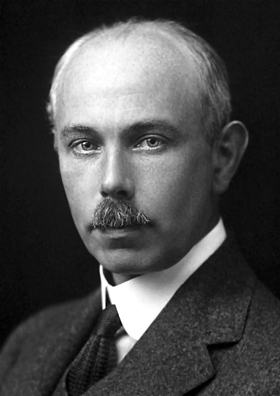
\includegraphics[width=\linewidth]{images/book3/aston.jpg}
\end{minipage}\hspace{0.02\linewidth}%
\begin{minipage}[t]{0.24\linewidth}
\vspace{0pt}
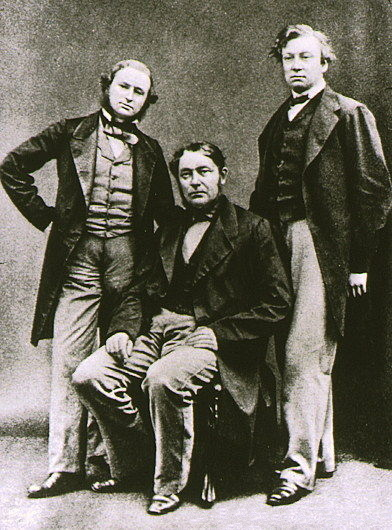
\includegraphics[width=\linewidth]{images/book3/kirchhoff-bunsen.jpg}
\end{minipage}\hfill
\begin{minipage}[t]{0.54\linewidth}
\vspace{0pt}
بيّن غوستاف كيرشوف وروبرت بنزن نحو سنة 1860 أن لكل عنصر خطوطه الخاصة في اللهب،
واكتشفا السيزيوم والروبيديوم بخطوطهما المجهولة. وبيّن مطياف الكتلة الذي صنعه فرانسيس أستون، منذ
1919، أن معظم العناصر خلائط من النظائر؛ ونال جائزة نوبل في الكيمياء سنة 1922.
(صور: أستون، مؤلف مجهول، ملكية عامة؛ وكيرشوف وبنزن وهنري روسكو سنة 1862، من
مجموعة روسكو، ملكية عامة؛ ويكيميديا كومنز.)
\end{minipage}
\end{history}

\section{تمارين}

\begin{exercise}[$\star$]\label{exo:b2:mass-spec-atomic:1}
أعطِ $m/z$ لما يأتي: \omterm{def:b2:mass-spec-atomic:molecular-ion}{الأيون الجزيئي} للبنزين \ce{C6H6}؛ وأيون كتلته \qty{400}{u} يحمل
شحنتين؛ والجزيء المبرتن للكافيين (\ce{C8H10N4O2}، كتلته الاسمية 194) المتكوّن بالرذاذ الكهربائي.
\end{exercise}

\begin{exercise}[$\star$]\label{exo:b2:mass-spec-atomic:2}
لمركب من C وH وN وO \omterm{def:b2:mass-spec-atomic:molecular-ion}{أيون جزيئي} عند $m/z$ 73. ماذا يمكن قوله عن ذرات النيتروجين فيه؟
واقترح صيغة.
\end{exercise}

\begin{exercise}[$\star$]\label{exo:b2:mass-spec-atomic:3}
تُظهر مجموعة \omterm{def:b2:mass-spec-atomic:molecular-ion}{أيون جزيئي} قمتين تفصل بينهما وحدتان، متقاربتي الارتفاع. وتُظهر أخرى قمتين
تفصل بينهما وحدتان بالنسبة 3 : 1. أي الهالوجينات؟
\end{exercise}

\begin{exercise}[$\star$]\label{exo:b2:mass-spec-atomic:4}
ملح يلوّن اللهب بالأصفر؛ وآخر بالأحمر القرمزي. حدّد العنصرين وأعطِ الأطوال الموجية
لخطوطهما.
\end{exercise}

\begin{exercise}[$\star\star$]\label{exo:b2:mass-spec-atomic:5}
لهيدروكربون القمة $M$ عند 100 \% و$M+1$ عند 6.7 \%. كم ذرة كربون فيه؟
\end{exercise}

\begin{exercise}[$\star\star$]\label{exo:b2:mass-spec-atomic:6}
احسب الكتل الدقيقة للجزيئات \ce{CO} و\ce{N2} و\ce{C2H4} وقدرة الميز اللازمة لفصل
كل زوج.
\end{exercise}

\begin{exercise}[$\star\star$]\label{exo:b2:mass-spec-atomic:7}
يُظهر طيف EI للبنتان-3-ون قممًا عند 86 و57 (\omterm{def:b2:mass-spec-atomic:spectrum}{قمة الأساس}) و29. انسبها.
\end{exercise}

\begin{exercise}[$\star\star$]\label{exo:b2:mass-spec-atomic:8}
يُظهر طيف البنتان-2-ون قممًا عند 86 و71 و58 و43 (\omterm{def:b2:mass-spec-atomic:spectrum}{قمة الأساس}). انسبها، وفسّر
لماذا لا يُظهر البنتان-3-ون إلا قمة صغيرة عند 58.
\end{exercise}

\begin{exercise}[$\star\star$]\label{exo:b2:mass-spec-atomic:9}
تعطي معايير النحاس عند 1.0 و2.0 و3.0 و\qty{4.0}{mg/L} الامتصاصيات 0.052 و0.104 و0.155 و0.207؛
وتعطي عينة 0.128 (معطيات تمرين). احسب تركيز النحاس فيها.
\end{exercise}

\begin{exercise}[$\star\star\star$]\label{exo:b2:mass-spec-atomic:10}
في محلل زمن الطيران، $L = \qty{1.00}{m}$ و$U = \qty{20.0}{kV}$. احسب زمن طيران
أيون أحادي الشحنة كتلته \qty{1000}{u}، والزمن الفاصل بينه وبين أيون كتلته \qty{1001}{u}.
\end{exercise}

\begin{exercise}[$\star\star\star$]\label{exo:b2:mass-spec-atomic:11}
احسب مجموعة \omterm{def:b2:mass-spec-atomic:molecular-ion}{الأيون الجزيئي} لثنائي كلوروميثان، \ce{CH2Cl2}: قيم $m/z$ والشدات
النسبية.
\end{exercise}

\begin{exercise}[$\star\star\star$]\label{exo:b2:mass-spec-atomic:12}
في ICP-MS، يتداخل \ce{^{40}Ar^{16}O+} مع \ce{^{56}Fe+}. احسب قدرة الميز اللازمة
لفصلهما، واقترح مخرجًا آخر.
\end{exercise}

\section{مسألة: هاليد مجهول}

\begin{problem}[{مسألة نهاية الأسبوع --- مجموعة أيون جزيئي مع الكلور والبروم، وعدد
ذرات الكربون، والشظايا، وبنية يُتحقق منها مقابل كل قمة}]
\label{pb:b2:mass-spec-atomic:1}
سائل عديم اللون، يخرج قمةً واحدة في \omterm{def:b2:chromatography:techniques}{كروماتوغرافيا الغاز}، يعطي طيف كتلة EI أدناه (بيانات
قاعدة NIST الشبكية). القمم الرئيسية ($m/z$: الشدة النسبية): 156: 14.5؛ 157: 0.5؛ 158: 18.6؛ 159: 0.6؛ 160:
4.4؛ 107: 6.7؛ 109: 6.3؛ 93: 3.3؛ 95: 2.9؛ 77: 59؛ 79: 18.7؛ 76: 39.5؛ 49: 12.9؛ 51: 4.3؛ 41: 100؛ 39:
26.2؛ 27: 24.6. الوفرات النظائرية: \ce{^{35}Cl} 0.758، \ce{^{37}Cl} 0.242، \ce{^{79}Br} 0.5069،
\ce{^{81}Br} 0.4931، \ce{^{12}C} 0.989، \ce{^{13}C} 0.011.
% ledger: ms:bromochloropropane, iso:Cl35, iso:Cl37, iso:Br79, iso:Br81, iso:C12, iso:C13, mass:C12, mass:H1, mass:Br79, mass:Cl35

\begin{center}
\begin{tikzpicture}
\begin{axis}[width=0.8\linewidth, height=4.6cm, xmin=20, xmax=170, ymin=0, ymax=112,
  xlabel={$m/z$}, ylabel={\foreignlanguage{arabic}{الشدة النسبية}}, label style={font=\small},
  tick label style={font=\scriptsize}, ycomb, xtick={27,41,49,77,93,107,122,156}]
\addplot[omDef, thick] table[x=mz, y=I] {figdata/out/bachelor-2-mass-spectra-d.dat};
\end{axis}
\end{tikzpicture}
\end{center}
% figdata: bachelor-2/mass-spectra.py part d

\medskip
\noindent\textbf{الجزء الأول --- \omterm{def:b2:mass-spec-atomic:molecular-ion}{الأيون الجزيئي}.}
\begin{enumerate}
  \item أي القمم تكوّن مجموعة \omterm{def:b2:mass-spec-atomic:molecular-ion}{الأيون الجزيئي}؟ ولماذا ليست قمة واحدة؟
  \item أي الهالوجينات توحي بها مجموعة من ثلاث قمم تفصل بينها وحدتان؟
  \item ما الكتلة الاسمية لأخف صورة نظائرية؟
  \item ماذا تقول \omterm{def:b2:mass-spec-atomic:nitrogen-rule}{قاعدة النيتروجين}؟
  \item اطرح \ce{^{79}Br} واحدًا و\ce{^{35}Cl} واحدًا: ماذا يبقى، وأي شظية هيدروكربونية
        لها تلك الكتلة؟
  \item اقترح صيغة جزيئية وأعطِ درجة عدم تشبعها.
\end{enumerate}

\medskip
\noindent\textbf{الجزء الثاني --- ذرات الكربون والكتلة الدقيقة.}
\begin{enumerate}[resume]
  \item من النسبة 157/156، قدّر عدد ذرات الكربون.
  \item لماذا يكون هذا التقدير تقريبيًا هنا؟
  \item أي الصور النظائرية تساهم في القمة عند 158؟
  \item احسب \omterm{def:b2:mass-spec-atomic:exact-mass}{الكتلة الأحادية النظير} \omterm{def:b2:mass-spec-atomic:molecular-ion}{للأيون الجزيئي}.
  \item للمركب \ce{C10H20O} أيضًا كتلة اسمية 156 (الدقيقة 156.151). أي قدرة ميز تفصل
        بينهما؟
  \item هل \omterm{def:b2:mass-spec-atomic:molecular-ion}{للأيون الجزيئي} لمركب فيه رابطة C=C والهالوجينات نفسها كتلة
        اسمية مختلفة؟
\end{enumerate}

\medskip
\noindent\textbf{الجزء الثالث --- الشظايا.}
\begin{enumerate}[resume]
  \item الزوج 77/79 بالنسبة 3 : 1. أي ذرة فُقدت، وما الأيون؟
  \item فسّر القمة عند 76.
  \item انسب \omterm{def:b2:mass-spec-atomic:spectrum}{قمة الأساس} عند 41.
  \item انسب الزوج 49/51.
  \item انسب الزوجين 93/95 و107/109.
  \item لماذا تُفقد ذرة البروم بسهولة أكبر من ذرة الكلور؟
  \item كان 1-برومو-1-كلوروبروبان سيعطي \ce{CHBrCl+} عند 127 و129 و131. هل يدعمه
        الطيف؟
\end{enumerate}

\medskip
\noindent\textbf{الجزء الرابع --- البنية.}
\begin{enumerate}[resume]
  \item اقترح البنية.
  \item تحقق من أنها تفسر كل قمة مذكورة.
  \item هل يمكن أن تحدث \omterm{def:b2:mass-spec-atomic:fragmentation}{إعادة ترتيب ماكلافرتي}؟ ولماذا؟
  \item ارسم المتماكب الذي كان سيعطي قمة قوية عند $m/z$ 63/65 ولا شيء عند 49/51.
  \item أي الصور النظائرية تصنع القمة عند 160؟
  \item من الوفرات النظائرية، احسب نسبة القمم $M$ و$M+2$ و$M+4$ لكلور
        واحد وبروم واحد، وقارنها بالطيف.
\end{enumerate}
\end{problem}
